\documentclass[12pt,oneside]{report}
\usepackage[utf8]{inputenc}
\usepackage{graphicx}
\graphicspath{ {images/} }
\usepackage{caption}
\usepackage{subcaption}
\usepackage[a4paper,width=150mm,top=25mm,bottom=25mm,bindingoffset=6mm]{geometry}
\usepackage{fancyhdr}
\pagestyle{fancy}
\fancyhead{}
\fancyhead[RO,LE]{Water Monitoring}
\fancyfoot{}
\fancyfoot[LE,RO]{\thepage}
\fancyfoot[LO,CE]{Chapter \thechapter}
\fancyfoot[CO,RE]{Tarun Kantiwal}
\renewcommand{\headrulewidth}{0.4pt}
\renewcommand{\footrulewidth}{0.4pt}
\usepackage{tikz}
\usetikzlibrary{fit, positioning}
\usepackage{lipsum}
\usepackage{hyperref}
\bibliographystyle{ieeetr}
\usepackage{biblatex}
\addbibresource{references.bib}


\usepackage{listings}
\usepackage{xcolor} % for setting colors

% set the default code style
\lstset{
    frame=tb, % draw a frame at the top and bottom of the code block
    tabsize=4, % tab space width
    showstringspaces=false, % don't mark spaces in strings
    numbers=left, % display line numbers on the left
    commentstyle=\color{green}, % comment color
    keywordstyle=\color{blue}, % keyword color
    stringstyle=\color{red} % string color
}



\begin{document}

%TC:ignore
\begin{titlepage}
    \begin{center}
        \vspace*{0.1cm}
        
          
        
\includegraphics[width=0.6\textwidth]{images/SecondaryLogo.png}
        
        \large
         \textbf{Department of Computer Science}
         \vspace{1cm}
         
         \textbf{B.Tech Computer Science}
         \vspace{1cm}
         
         Academic Year 2020 - 2021
         
         
         \vspace{2cm}
        
        
        \LARGE
        \textbf{Prediction of Dissolved Oxygen from pH and Water Temperature in Aquaculture Prawn Ponds}
        
        
        \vspace{1.5cm}
        \large
        \textbf{Tarun Kantiwal}
        
        (COE17B031)\\
        Under\\
        \large
        \textbf{Dr. Munesh Pal Singh}
        
        
       % \vfill
        \vspace{1.5cm}
        A report submitted to describe my summer intership work \\and to present in internship panel

        
        \vspace{0.8cm}
      \begin{flushright}
        \footnotesize
        IIITDM Kancheepuram \\
        Department of Computer Science\\
        Vandalur-Kelambakkam Road\\
        Chennai-127\\
        Tamil Nadu\\
        India \\
        T: +91-44-2747 6300\\
        F: +91-44-2747 6301\\
        \end{flushright}
        
    \end{center}
\end{titlepage}

\thispagestyle{plain}

\textbf{Abstract}

\vspace{1cm}
This report describes my internship experience at the Indian Information of Information Technology Design and Manufacturing in
Kancheepuram , and it is divided into four chapters.\\

Chapter One summarizes the projects and It gives us the introduction and need of the project.\\

Chapter Two dealt with the idea of IoT in the project to send data to cloud and and make use of the data for further calculations.\\

Chapter Three provides how to and what to do with data over the cloud and project is to handle data to make inferences (Machine Learning or Cleaning data).\\

Chapter Four Dealt with the Back end or hosting server and make prediction online using API the work done in Nodejs.\\

Chapter Five In this chapter we will finally done our work for web App and Mobile Application for end user.



\chapter*{Acknowledgements}
Working on this project is very good experience of me. During these five month internship i learned a lot and all my courses made equal and big contribution in completing this internship, Internet of things, Programming, Data cleaning and all maths courses helped me a lot.\\

I want to help Dr. Munesh Pal Singh to help me throughout the project by providing me knowledge about IoT and keep me calm in while solving error or when i feel stuck in some difficult situation\\

Further on I want to thank stackoverflow, github and all programming site because these community helped me a lot while i stuck in error regarding cloud, Web App, Mobile App, Tensorflow Model for web and App. 



\vspace{3cm}

\begin{tikzpicture}[
    node distance = 0mm and 1mm,
box/.style = {text width=15cm, font=\normalsize},  % define nodes style
                    ]
\node (n1) [box,draw] {I certify that the work presented in the dissertation is my own unless referenced.\\
\vspace{1cm}
%replace the image signature_example with your own image of your signature
Signature: 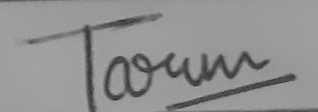
\includegraphics[width=0.2\textwidth]{images/image.png}\\ 
\vspace{1cm}
Date: 14/Oct/2020
\vspace{1cm}
};
\end{tikzpicture}

\tableofcontents

% \listoffigures

% \listoftables

%TC:endignore

\chapter{Introduction}

A crucial activity in prawn farming is monitoring prawn pond water quality. Variables such as dissolved oxygen (DO), pH, temperature, and salinity are commonly monitored using sensors Temp sensor pH sensor and many other sensor are widely used by small farmers and pond owner to monitor water quality for fishes and agriculture related work. Sensor monitoring comes with challenges such as: purchasing and main- taining sensors is costly, gathering readings with hand-held sensors over many ponds is time consuming, readings can be incorrectly logged, and sensors can fail. Such problems can be mitigated by reducing the number of sensors required. A sensor can be made redundant if its associated variable can be predicted from other sensor data In this study a recurrent neural network (RNN) , a linear regression model,are used to predict dissolved oxygen from pH and water temperature sensor readings.\\

Aquaculture consists of the set of activities, knowledge and techniques for the breeding of aquatic plants and some species of animals. This activity has a great importance in economic development and food production. Continuous monitoring of the physical, chemical and biological parameters of pond water helps not only to predict and control the negative conditions of aquaculture, but also to avoid environmental damage and the collapse of the production process. The monitoring of physical and chemical variables such as: oxygen, temperature and pH in water are vital to maintain adequate conditions and avoid undesirable situations that may lead to the collapse of aquaculture systems


\section{Aims and Objectives}

The aim of this project is to get the main factor of water Dissolved Oxygen get predict by some given properties of water using IoT solution and Machine Learning Model and made them accessible to end user without any hustle so that they can access in Mobile device like Application of iOS and Android and web App.\\


Here is the list of the necessary and complete set of objectives that we will need to achieve in order to satisfy our above listed aim using modern day technologies :. 

\begin{enumerate}
\item	Undertook a relevant background study to identify existing work in the area, and to identify appropriate techniques which can be adopted to produce a solution in this project. like is there any model which can help us to do thing easily 
\item	In the task first we have and we want data of temp and ph so that we can make a prediction of dissolved oxygen but before making prediction data cleaning we need to done change format like json and other compatible with mobile app or web app.
\item	We have to implement one Tensorflow model by which we can make prediction and calculate approximated output given any particular input we have to use Tensorflow Lite (For Mobile App Development ) and Tensorflow.js for web app Development.
\item	Next thing we need to do is get data from pond in real time and upload all neccessary data like pH and Temp to make prediction using Internet of things example Arduino UNO is perfect to use data and Wifi module to upload data on cloud. Search for free cloud provider is challeging because no one provide free service
\item	After getting model ready and data uploaded to cloud we have to make data accessible to end user like farmer and fish farmer so that they can use prediction to make aquatic and agriculture life better. So for this purpose we have to make one Web App and Mobile App with very easy interface so everybody can use it.
\item	In Last all the blocks are ready now we have to combine them all and make one final product which can make good predictions.
\end{enumerate}


\section{Project Approach}

The Project will used many new and advanced technology which will make good and better product finally and which will make significant impact on society so we will follow all the above aim and make final product good as all the technology we will use are new so we have to handle thing by learning and doing. Tensorflow is very good for advanced Machine Learning thing and Java Script is good for web and cross platform native mobile application. The problem which we will face is that the data which we are using is having the temperature between 25-31$^{\circ}$C and ph is of normal water (6-8) so, making prediction out of this bound will give us error in prediction like for very cold water (o-10 $^{\circ}$C) it will give error as we have to collect more data in this range and train the model again but it will not be difficult task as we will get data any time soon after this Lock Down end. We have to host one prediction server which will make online prediction using API. 

\section{Dissertation Outline}

Below is the task and the chapter in which detailed description of each task is included chapter wise and summary of the chapter included in Dissertation Outline.\\


Chapter 1, already talk about what the project is all about where IoT and Machine Learning and Web Model will be used.\\


Chapter 2, In chapter two we will Talk about Iot and Cloud data handeling.  \\

Chapter 3, Data Computation, cleaning and make inference from data for predictions.


Chapter 4, Talk about Api which will be user for Mobile App and web app.\\


Chapter 5, One website and Mobile app will be used for Desktop and Mobile Users.\\

Chapter 6, It shows about out testing and App and web App for are all the things working fine ?\\

Chapter 7, Conclusion of our Work and Future.

\chapter{IoT and Cloud}
\section{IoT and Cloud Introduction}
The Internet of Things (IoT) involves the internet-connected devices we use to perform the processes and services that support our way of life. Another component set to help IoT succeed is cloud computing, which acts as a sort of front end. Cloud computing is an increasingly popular service that offers several advantages to IoT, and is based on the concept of allowing users to perform normal computing tasks using services delivered entirely over the internet.\\

Iot in cloud offers public cloud services can easily help the IoT area, by providing third party access to the infrastructure. Hence, the integration can help IoT data or computational components operating over IoT devices.\\

IoT devices need a lot of storage to share information for valuable purposes. Iot in cloud, like the StoneFly Cloud Connect to Microsoft Azure or we will use ThinkSpeak a free cloud service for IoT for student projects can provide customers with greater space which can increase as per the users demand. Helping to resolve the storage needs of customers.\\

The large amounts of data produced by IoT devices need extreme performance to interact and connect with one another. Iot in cloud provides the connectivity which is necessary to share information between the devices and make meaning from it at a fast pace.\\

Internet Cloud Computing infrastructures help IoT to give meaning to the greater amount of data generated. Users have no worry of buying greater or less storage. They can easily scale the storage as the data generated increases and pay for the amount of storage they consume with Internet Cloud Computing.




\section{IoT in Project}
he aim of this work is design and implements a distributed system for aquaculture water quality care through remote monitoring of dissolved oxygen, pH and temperature. This work will contribute remote monitoring distributed system through what is known as the Internet of Things to monitoring water quality in ponds. The system is modular, portable, low cost, versatile and allows sharing information through the cloud that can be used for the development and improvement of aquaculture activities. \\

The system can be implemented in aquaculture farms to be able to monitor in real time the most important physical-chemical variables of the water. With this having a faster response with respect to what actions to take when conditions arise in the water quality of the ponds\\

A monitoring system for water quality in aquaculture ponds is mentioned in the publication A Mobile Platform for Remote Monitoring of Water Quality. Mobile sensor platform for monitoring ponds. This system consists of the following architecture. It has the sensing node of each pond connected to a sink; this sink sends the information to a mobile application to have a visualization of the data in real time. This information is transmitted via GSM / 3G to the Internet, it can be monitored remotely and the information is stored in a database. In the results the data of the ponds were shown remotely and the measures were corroborated by the transport staff.\\


\section{Work Flow or Connectivity}

Here is the diagram which will help us to understand our work flow. Here is the images of all the sensors we will use.\\

pH Sensor : -\\

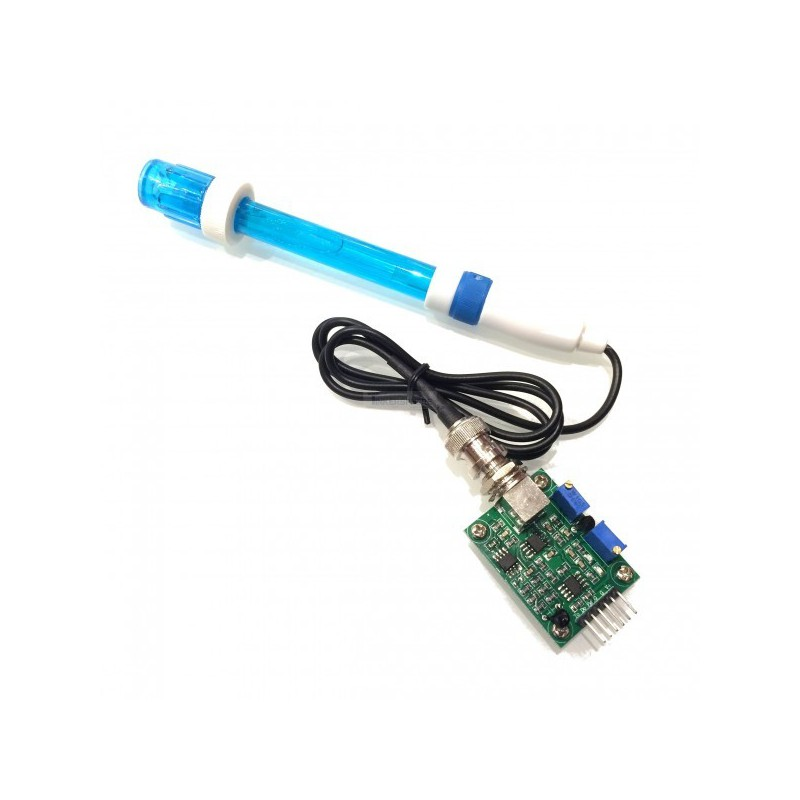
\includegraphics[width=0.6\textwidth]{images/ph sensor.jpg}\\

Temperature Sensor : -\\

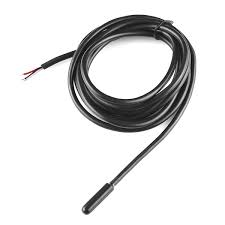
\includegraphics[width=0.6\textwidth]{images/temp sensor.jpeg}
\\

Work Flow Diagram :- \\

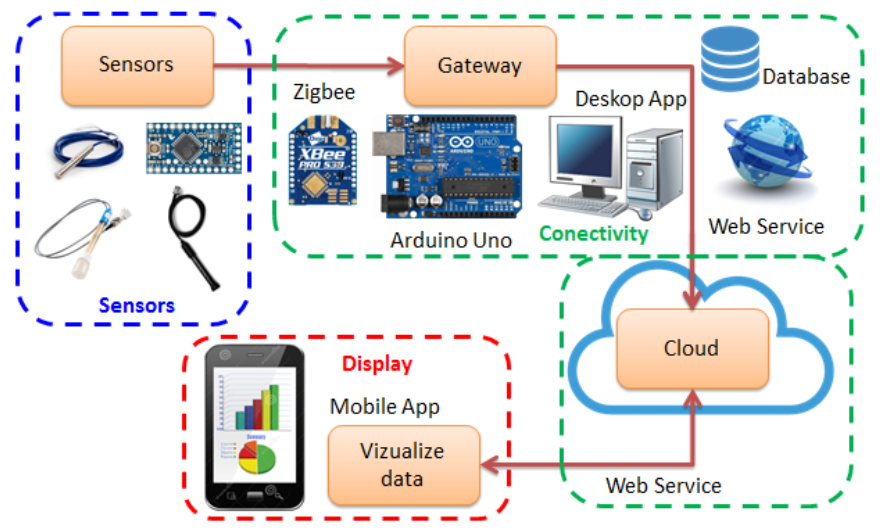
\includegraphics[width=0.6\textwidth]{images/workflow.png}\\



\subsection{Collect Data From Sensor}

In this section we will talk about first task of our workflow collect data from sensor and log it to console of arduino UNO. later we will send it to Cloud (ThinkSpeak for entire Project).\\

Below is the code of Collecting ph sensor and its connection and console it to COM Port console.\\

Figure : - 

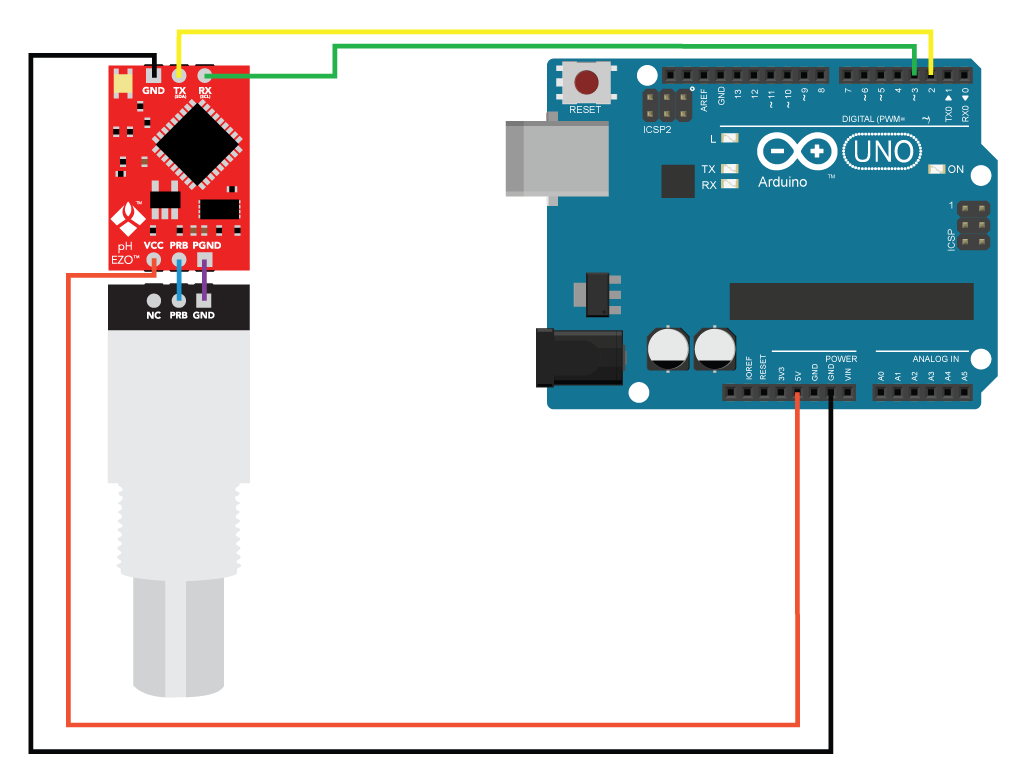
\includegraphics[width=0.6\textwidth]{images/ph-probe-calibration-wiring-diagram_YLRPvVdUwm.png}\\


\begin{lstlisting}[language=C++, caption={Arduino code for Ph sensor data}]
#include <Wire.h>
#include <LiquidCrystal_I2C.h>
LiquidCrystal_I2C lcd(0x27, 16, 2);
float calibration_value = 21.34;
int phval = 0; 
unsigned long int avgval; 
int buffer_arr[10],temp;
void setup() 
{
 Serial.begin(9600);
  lcd.init(); 
  lcd.begin(16, 2);
  lcd.backlight();
  lcd.setCursor(0, 0);
  lcd.print("   Welcome to      ");
  lcd.setCursor(0, 1);
  lcd.print(" Circuit Digest    ");
  delay(2000);
  lcd.clear();
}
void loop() {
 for(int i=0;i<10;i++) 
 { 
 buffer_arr[i]=analogRead(A0);
 delay(30);
 }
 for(int i=0;i<9;i++)
 {
 for(int j=i+1;j<10;j++)
 {
 if(buffer_arr[i]>buffer_arr[j])
 {
 temp=buffer_arr[i];
 buffer_arr[i]=buffer_arr[j];
 buffer_arr[j]=temp;
 }
 }
 }
 avgval=0;
 for(int i=2;i<8;i++)
 avgval+=buffer_arr[i];
 float volt=(float)avgval*5.0/1024/6;
 float ph_act = -5.70 * volt + calibration_value;
 lcd.setCursor(0, 0);
 lcd.print("pH Val:");
 lcd.setCursor(8, 0);
 lcd.print(ph_act);
 delay(1000);
}
\end{lstlisting}\\


Below is the code of Collecting temp. sensor and its connection and console it to COM Port console.\\

Figure : - 

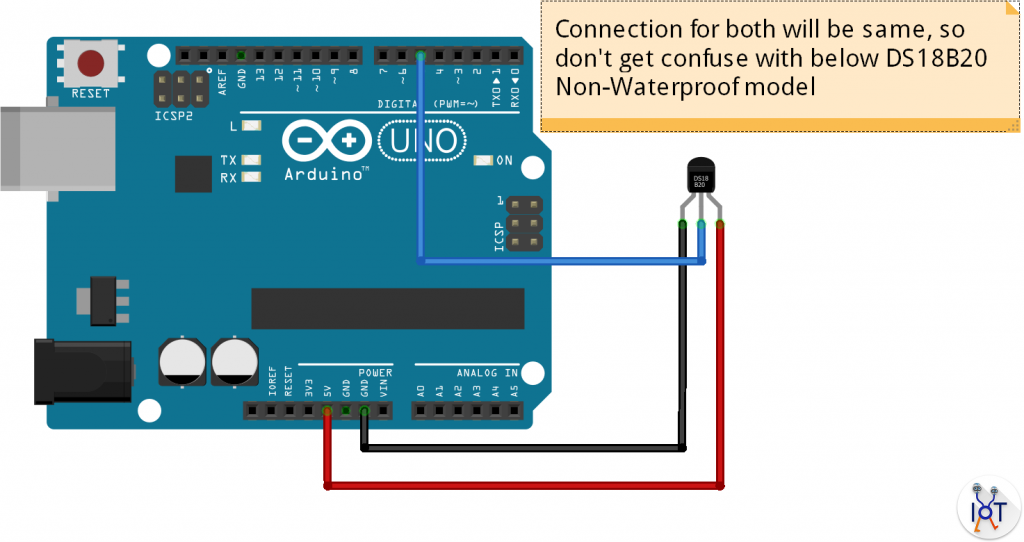
\includegraphics[width=0.6\textwidth]{images/temparature_sensor-www_iotboys_com_-1024x542_LqdcDeudhb.png}\\

\begin{lstlisting}[language=C++, caption={Arduino code for temp. sensor data}]
/********************************************************************/
// First we include the libraries
#include <OneWire.h> 
#include <DallasTemperature.h>
/********************************************************************/
// Data wire is plugged into pin 2 on the Arduino 
#define ONE_WIRE_BUS 2 
/********************************************************************/
// Setup a oneWire instance to communicate with any OneWire devices  
// (not just Maxim/Dallas temperature ICs) 
OneWire oneWire(ONE_WIRE_BUS); 
/********************************************************************/
// Pass our oneWire reference to Dallas Temperature. 
DallasTemperature sensors(&oneWire);
/********************************************************************/ 
void setup(void) 
{ 
 // start serial port 
 Serial.begin(9600); 
 Serial.println("Dallas Temperature IC Control Library Demo"); 
 // Start up the library 
 sensors.begin(); 
} 
void loop(void) 
{ 
 // call sensors.requestTemperatures() to issue a global temperature 
 // request to all devices on the bus 
/********************************************************************/
 Serial.print(" Requesting temperatures..."); 
 sensors.requestTemperatures(); // Send the command to get temperature readings 
 Serial.println("DONE"); 
/********************************************************************/
 Serial.print("Temperature is: "); 
 Serial.print(sensors.getTempCByIndex(0)); // Why "byIndex"?  
   // You can have more than one DS18B20 on the same bus.  
   // 0 refers to the first IC on the wire 
   delay(1000); 
} 
\end{lstlisting}\\

\subsection{Send data to cloud (ThingsSpeak)}

In this section we will make use of the data which we collected using both the sensor temp and ph and upload that data into the ThingsSpeak cloud which is cloud service offer by Matlab and it is free for student if you use it in limited conditions like minimum request to send data.\\

And from above section we know that the data from arduino is very fast reading like we get in every millisecond but we will upload data in 1 minute interval in cloud. to make minimum free usage for cloud.\\

Now Next thing which we will need to do to upload data in cloud is that we will need one wifi module which will connect to near by wifi hotspot and connect to cloud api to send data to channels in cloud. Below is the image of esp module device and code which make a connection of arduino and cloud\\

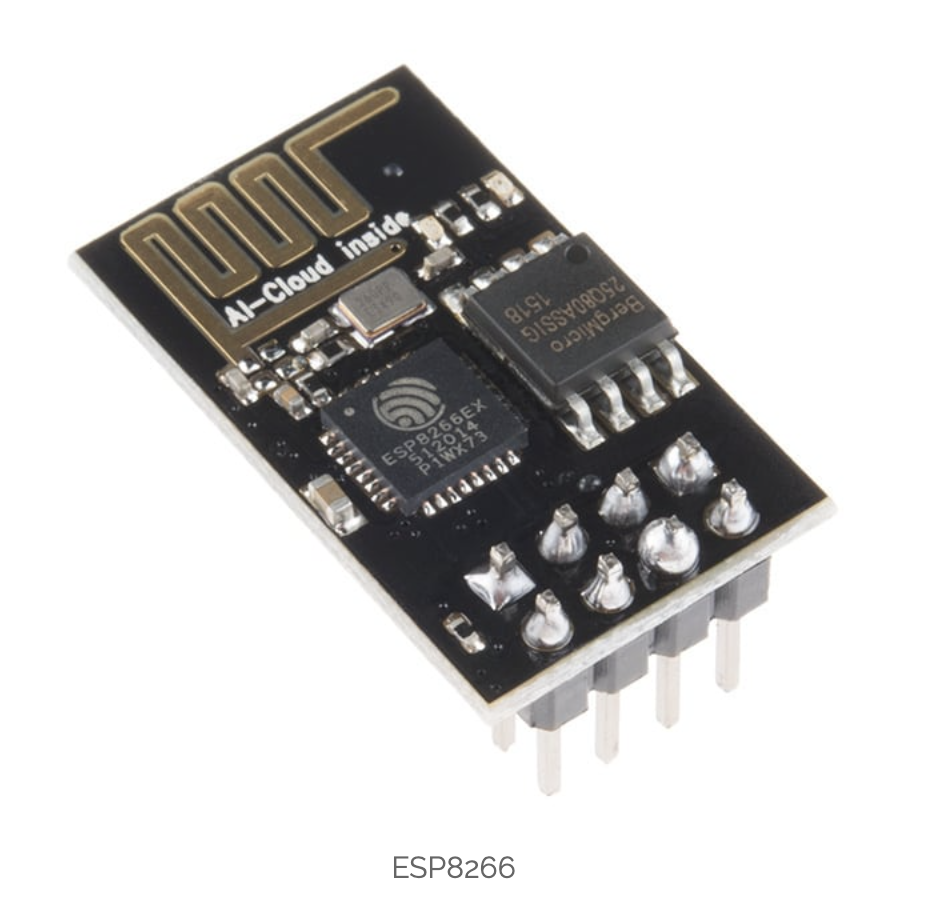
\includegraphics[width=0.6\textwidth]{images/esp.png}\\

\begin{lstlisting}[language=C++, caption={Arduino code for sending data to cloud}]

#include "ThingSpeak.h"
#include <ESP8266WiFi.h>

//------- WI-FI details ----------//
char ssid[] = "xxxxxxxxx"; //SSID here
char pass[] = "yyyyyyyyy"; // Passowrd here
//--------------------------------//

//----------- Channel details ----------------//
unsigned long Channel_ID = 12345; // Your Channel ID
const char * myWriteAPIKey = "ABCDEF12345"; //Your write API key
//-------------------------------------------//

const int Field_Number_1 = 1;
const int Field_Number_2 = 2;
String value = "";
int value_1 = 0, value_2 = 0;
int x, y;
WiFiClient  client;

void setup()
{
  Serial.begin(115200);
  WiFi.mode(WIFI_STA);
  ThingSpeak.begin(client);
  internet();
}

void loop()
{
  internet();
  if (Serial.available() > 0)
  {
    delay(100);
    while (Serial.available() > 0)
    {
      value = Serial.readString();
      if (value[0] == '*')
      {
        if (value[5] == '#')
        {
          value_1 = ((value[1] - 0x30) * 10 + (value[2] - 0x30));
          value_2 = ((value[3] - 0x30) * 10 + (value[4] - 0x30));
        }
      }
    }
  }
  upload();
}

void internet()
{
  if (WiFi.status() != WL_CONNECTED)
  {
    while (WiFi.status() != WL_CONNECTED)
    {
      WiFi.begin(ssid, pass);
      delay(5000);
    }
  }
}

void upload()
{
  ThingSpeak.writeField(Channel_ID, Field_Number_1, value_1, myWriteAPIKey);
  delay(15000);
  ThingSpeak.writeField(Channel_ID, Field_Number_2, value_2, myWriteAPIKey);
  delay(15000);
  value = "";

}

\end{lstlisting}\\

\subsection{Conclusion}

Now all data that we will need to make real time prediction is uploaded in cloud now we have to fetch data from this cloud and implement in mobile app and web app but before that we have to train our tensorflow model to make good model which can give us best predictions from our data. So, in the next section we will use Tensorflow Numpy Pandas and scikit to make prediction.

\chapter{Methodology (Or Approach)}
In this section we will talk about cleaning data using pandas and convert clean csv data into json using online csv to json converter and we will use sci-kit and tensorflow for two machine learning model Linear Regression and Artificial Neural Network in both Tensorflow and Sci-kit and later we will decide which model to use. In below subsection. first we will write little description of Data Cleaning and ML.\\

\section{Data Cleaning}

Data cleaning is the process of preparing data for analysis by removing or modifying data that is incorrect, incomplete, irrelevant, duplicated, or improperly formatted. This data is usually not necessary or helpful when it comes to analyzing data because it may hinder the process or provide inaccurate results. There are several methods for cleaning data depending on how it is stored along with the answers being sought. Data cleaning is not simply about erasing information to make space for new data, but rather finding a way to maximize a data set’s accuracy without necessarily deleting information. For one, data cleaning includes more actions than removing data, such as fixing spelling and syntax errors, standardizing data sets, and correcting mistakes such as empty fields, missing codes, and identifying duplicate data points. Data cleaning is considered a foundational element of the data science basics, as it plays an important role in the analytical process and uncovering reliable answers. Most importantly, the goal of data cleaning is to create data sets that are standardized and uniform to allow business intelligence and data analytics tools to easily access and find the right data for each query.

\subsection{Pandas and Numpy}

For the purpose of data cleaning we will use Pandas and Numpy as it is very easy to handle data in pandas dataframes and Numpy lib in python is very good library to handle array and manipulate array using advanced array methods.\\

In this Project we have csv data of water with following properties\\

STATION CODE,LOCATIONS,STATE,Temp,D.O. (mg/l),PH,CONDUCTIVITY (µmhos/cm),B.O.D. (mg/l),NITRATENAN N+ NITRITENANN (mg/l),FECAL COLIFORM (MPN/100ml),TOTAL COLIFORM (MPN/100ml)Mean,year.\\


But the problem with this data is that the temp, ph and D.o is having some values which is not in scale and for example ph above 14 and and have value NAN in the temp, ph etc and the which we will need only temperature, ph and dissolved oxygen for our project so we will get all these clean data in new csv.

\subsection{Machine Learning and Prediction}

Machine learning is an application of artificial intelligence (AI) that provides systems the ability to automatically learn and improve from experience without being explicitly programmed. Machine learning focuses on the development of computer programs that can access data and use it learn for themselves.\\


The process of learning begins with observations or data, such as examples, direct experience, or instruction, in order to look for patterns in data and make better decisions in the future based on the examples that we provide. The primary aim is to allow the computers learn automatically without human intervention or assistance and adjust actions accordingly.\\

Below is the code of Predictions using Our data using Tensorflow and Sci-kit Learn and data clearning in pandas also done in same code.\\

\begin{lstlisting}[language=python, caption={Linear regression Model Scikit}]

import numpy as np
import pandas as pd
import matplotlib.pyplot as plt

dataset = pd.read_csv("waterdata.csv", encoding= 'unicode_escape')

dataset.describe()

dataset["Temp"] = pd.to_numeric(dataset['Temp'], errors='coerce')
dataset["Temp"] = dataset["Temp"].replace(np.nan, 0)
dataset["PH"] = pd.to_numeric(dataset['PH'], errors='coerce')
dataset["PH"] = dataset["PH"].replace(np.nan, 0)
dataset["D.O. (mg/l)"] = pd.to_numeric(dataset['D.O. (mg/l)'], errors='coerce')
dataset["D.O. (mg/l)"] = dataset["D.O. (mg/l)"].replace(np.nan, 0)
# dataset["Temp"] = dataset["Temp"].fillna()

y = dataset["D.O. (mg/l)"]

X = dataset[["Temp", "PH"]]

# X["Temp"] = X["Temp"].mean()
# X["Temp"] = X[X["Temp"]==0].mean()

# X["Temp"].mean()
X["PH"].mean()

dataset=dataset.mask(dataset["Temp"]==0).fillna(dataset["Temp"].mean())
dataset=dataset.mask(dataset["PH"]==0).fillna(dataset["PH"].mean())
dataset=dataset.mask(dataset["D.O. (mg/l)"]==0).fillna(dataset["D.O. (mg/l)"].mean())

y = dataset["D.O. (mg/l)"]
X = dataset[["Temp", "PH"]]
X["PH"]

from sklearn.model_selection import train_test_split

X_train, X_test, y_train, y_test = train_test_split(X, y, test_size=0.3, random_state=101)

from sklearn.linear_model import LinearRegression

lm = LinearRegression()

lm.fit(X_train, y_train)

lm.coef_

predictions = lm.predict(X_test)

# predictions
# 0.07 0.0000032

X_test.shape

data = {'longitude':  [30.6],
        'latitude': [7.5]}

df = pd.DataFrame (data, columns = ['longitude','latitude'])

df.shape

answer = lm.predict(df)

answer


\end{lstlisting}\\

\begin{lstlisting}[language=python, caption={Linear regression Model Tensorflow API}]

# Commented out IPython magic to ensure Python compatibility.
import pandas as pd
import numpy as np
import matplotlib.pyplot as plt
import tensorflow as tf
plt.style.use("seaborn-colorblind")
# %matplotlib inline

used_features = ["Temp", "PH","D.O. (mg/l)"]
water = pd.read_csv('waterdata.csv', usecols = used_features, encoding= 'unicode_escape')
# m = pd.read_csv('waterdata.csv', encoding= 'unicode_escape')
# target["D.O. (mg/l)"] = m["D.O. (mg/l)"]
print(water.shape)
water.head()
# target.head()

water["Temp"] = pd.to_numeric(water['Temp'], errors='coerce')
water["Temp"] = water["Temp"].replace(np.nan, 0)
water["PH"] = pd.to_numeric(water['PH'], errors='coerce')
water["PH"] = water["PH"].replace(np.nan, 0)
water["D.O. (mg/l)"] = pd.to_numeric(water["D.O. (mg/l)"], errors='coerce')
water["D.O. (mg/l)"] = water["D.O. (mg/l)"].replace(np.nan, 0)

water=water.mask(water["Temp"]==0).fillna(water["Temp"].mean())
water=water.mask(water["PH"]==0).fillna(water["PH"].mean())
water=water.mask(water["D.O. (mg/l)"]==0).fillna(water["D.O. (mg/l)"].mean())

water

target = water["D.O. (mg/l)"]
features = water.drop('D.O. (mg/l)',axis=1)

features

target

from sklearn.model_selection import train_test_split
X_train, X_test, y_train, y_test = train_test_split(
     water, target, test_size=0.33, random_state=42)

# numeric_columns = ["Temp", "PH","D.O. (mg/l)"]
numeric_columns = ["Temp", "PH"]
X_train.drop('D.O. (mg/l)',axis=1, inplace=True)
X_test.drop('D.O. (mg/l)',axis=1, inplace=True)
X_test

numeric_features = [tf.feature_column.numeric_column(key = column) for column in numeric_columns]
print(numeric_features[0])

linear_features = numeric_features

training_input_fn = tf.compat.v1.estimator.inputs.pandas_input_fn(x=X_train, y=y_train, batch_size=32, shuffle=True, num_epochs=None)

eval_input_fn = tf.compat.v1.estimator.inputs.pandas_input_fn(x=X_test, y=y_test, batch_size=32, shuffle=False, num_epochs = 1)

linear_regressor = tf.estimator.LinearRegressor(feature_columns=linear_features,
                                                model_dir = "linear_regressor")

linear_regressor.train(input_fn = training_input_fn,steps=2000)

linear_regressor.evaluate(input_fn = eval_input_fn)

pred = list(linear_regressor.predict(input_fn = eval_input_fn))
pred = [p['predictions'][0] for p in pred]

prices = (pred)
print(prices)

X_test

y_test

predict_x = {
    'Temp': [30.1],
    'PH': [7.5],
}

def input_fn(features, batch_size=256):
    """An input function for prediction."""
    # Convert the inputs to a Dataset without labels.
    return tf.data.Dataset.from_tensor_slices(dict(features)).batch(10)

pred = linear_regressor.predict(
    input_fn=lambda: input_fn(predict_x))

pred

pred = [p['predictions'][0] for p in pred]

pred



\end{lstlisting}\\

\begin{lstlisting}[language=python, caption={ANN Model Tensorflow API}]


import pandas as pd
import numpy as np

used_features = ["Temp", "PH","D.O. (mg/l)"]
data = pd.read_csv("waterdata.csv", usecols = used_features, encoding= 'unicode_escape')

data

data["Temp"] = pd.to_numeric(data['Temp'], errors='coerce')
data["Temp"] = data["Temp"].replace(np.nan, 0)
data["PH"] = pd.to_numeric(data['PH'], errors='coerce')
data["PH"] = data["PH"].replace(np.nan, 0)
data["D.O. (mg/l)"] = pd.to_numeric(data["D.O. (mg/l)"], errors='coerce')
data["D.O. (mg/l)"] = data["D.O. (mg/l)"].replace(np.nan, 0)

data=data.mask(data["Temp"]==0).fillna(data["Temp"].mean())
data=data.mask(data["PH"]==0).fillna(data["PH"].mean())
data=data.mask(data["D.O. (mg/l)"]==0).fillna(data["D.O. (mg/l)"].mean())
target = data["D.O. (mg/l)"]

from sklearn.model_selection import train_test_split
X_train, X_test, y_train, y_test = train_test_split(
     data, target, test_size=0.33, random_state=42)

X_train.head()

train_X = X_train.drop(columns=['D.O. (mg/l)'])
train_X.head()

y_train.shape

train_y = data[['D.O. (mg/l)']]
train_y.head()

import tensorflow as tf
from tensorflow import keras
from tensorflow.keras import layers
import tensorflowjs as tfjs

n_cols = train_X.shape[1]

model = keras.Sequential(
    [
        layers.Dense(10, activation="relu", name="layer1",input_shape=(n_cols,)),
        layers.Dense(3, activation="relu", name="layer2"),
        layers.Dense(1, name="layer3"),
    ]
)

model.compile(optimizer='adam', loss='mean_squared_error')

from tensorflow.keras.callbacks import EarlyStopping

early_stopping_monitor = EarlyStopping(patience=3)

model.fit(train_X, train_y, validation_split=0.2, epochs=30, callbacks=[early_stopping_monitor])

tfjs_target_dir = "./tfjs"

tfjs.converters.save_keras_model(model, tfjs_target_dir)

test_X = X_test.drop(columns=['D.O. (mg/l)'])
test_X
# test_y_predictions = model.predict(X_test)

30.6,6.7,7.5

data = [[30.6, 7.5]] 
  
# Create the pandas DataFrame 
df = pd.DataFrame(data, columns = ['Temp', 'PH']) 
  
# print dataframe. 
df

# test_y_predictions = model.predict(test_X)
test_y_predictions = model.predict(df)

test_y_predictions


\end{lstlisting}\\

\subsection{Tensorflow or Sci-kit Which is Best ?}

When it's come to which model is best the answer is might complicated because which one is suitable for our App or website is the main reason to think about.\\

Sci-kit learn is a great library when it comes to simplicity and handling data sets on the other hand the tensorflow is slightly complicated because in tensorflow we have to deal with session to print and make calculation and also it deals with tensors so it is little bit difficult.\\

But Tensorflow is a great framework for machine learning enthusiast beacuse it provide vast variety of api which handle machine learning task easily. Tensorflow is easy can be used in mobile apps ans Website because of its great community and it is handled by google Below are the framework which are developed by tensorflow community\\

\begin{itemize}
  \item Tensorflow (Main Python Framework Widely used )
  \item Tensorflow.js (Use in Javascript web and app and node application)
  \item Tensorflow Lite (For Mobile compatibility)
\end{itemize}\\

So, Tensorflow is a great option, as it provide great API which we will need in this project in Mobile App and in Web App.\\

In this chapter we finished all the data handling cleaning, trained the machine learning model and exported them to make inferences from them in real time arduino data. Now we have to include them in React and iOS and Andriod Application.\\
\\
\\
\\
\\
\\
\\
\\

\\
\\
\\
\\
\\


\includegraphics[width=1\textwidth]{images/tensorflow.png}\\

\chapter{Design (Or What you did Part One)}
\input{chapters/chapter04}

\chapter{Implementation (Or What you did Part Two)}
\input{chapters/chapter04}

\chapter{Testing and Evaluation}
By Far our App and web app are working parfectly but we need to take care of some error and make app development and web much more effecient\\

Below are the Point which we need to be rectify

\section{Limited data}

These App uses water data which is very limited available and the data which is used in this whole project is downloaded from kaggle and that water data has some drawbacks

\begin{itemize}
  \item The Temperature data is in between normal temperature for example (23-30$^{\circ}$C) and if we make prediction below or above these temperature then we for sure will not get good predictions so we need more data of wide variety of temperature.
  \item And another point is of pH as we know all the water bodies which are pond lake all are not too much acidic and too much basic so when you make prediction for pH like 1-4 or basic solution like 10-14 then it will surely give error the trained model is not train for these temperature and pH ranges so we have to collect more data, to make good predictions
\end{itemize}

\section{Data Scaling and Best Model}

As the title suggest Data scaling and good model we already using best model for our mobile and web app but as we all know there are chances to minimize test error in machine learning we can improve model and make error minimum but we can't make error go away so we can always do work to reduce error and make our model accuracy very good\\

And Data scaling says while training data we can scale input to make predictions good this process is also the subset of above paragraph but these are two different task but interlinked so we have to take care of it\\



\chapter{Conclusion}
So here we are finishing all our work make a very vast machine learning Model and deployed them in Web App and iOS and android app and connected all the thing to cloud. So here are the things I acheive so far in this project

\begin{enumerate}
\item	I have completely met my aim and solved the problem
\item	 The Solution solved the problem as given by Dr. Munesh pal Singh
\item	The solution is although best for the certain most common temperature and pH range but for wide variety of data it is getting failed. so we have to rectify it
\end{enumerate}


\section{Future Work}
As we reached the end of our project but there are the task in chapter 6 which we have to do in Future to make this project more successful and great


\includegraphics[width=0.6\textwidth]{images/pond.png}\\




%TC:ignore
% \appendix
% \chapter{Personal Reflection }
% \input{chapters/appendixA}
% \chapter{Appendices}
% \input{chapters/appendixB}
% \chapter{Ethics approval}
% \input{chapters/appendixC}

% \printbibliography
%TC:endignore

\end{document}
